% Working draft; 6--8 page target. Full protocol figures remain in supplement.tex.
\documentclass[sigconf,nonacm]{acmart}
\setcopyright{none}
\settopmatter{printacmref=false,printccs=false,printfolios=true}
\acmDOI{}\acmISBN{}
\usepackage{booktabs}
\usepackage{graphicx}
\usepackage{adjustbox}
\setlength{\emergencystretch}{1em}
\title{Checking Semantic Correspondence Between Natural-Language and Lean Proofs}
\author{Taylor Belcher}
\author{ChatGPT}
\authornote{AI collaborator accessed through Codex; contributed implementation, experiment execution, literature retrieval, and drafting. Taylor Belcher directs the project.}
\renewcommand{\shortauthors}{Belcher and ChatGPT}
\begin{document}
\begin{abstract}
A Lean proof can establish a formal theorem without faithfully representing the English argument that accompanies it. We investigate whether language models can help identify this discrepancy, with an emphasis on assumptions, conclusions, and essential proof steps. Preliminary experiments with statement classifiers, synthetic proof swaps, random forests, and translation intermediaries produced strong scores on some constructed tasks but exposed weaknesses in evaluation data and generalization. A related-swap classifier reached 98.15\% accuracy on 54 held-out pairs, yet only 68.75\% on a small same-theorem diagnostic. Our main experiment separates Lean-to-English informalization from English-to-English comparison. We fine-tune Qwen3-14B with LoRA on 4,096 Herald pairs and use the original model as the judge. On 64 held-out pairs, the judge accepts 49 generated accounts; this is acceptance, not independently verified accuracy. A fresh ProofNet-trained informalizer scores 63.04\% on 46 of 54 related-swap test pairs, with eight generation-limit exclusions. Two targeted OpenAI cases both receive mismatch flags, but their explanations are confounded by omissions in the informalizations. The results motivate dependency-aware translation and public, human-reviewed datasets that label argument correspondence rather than only formal validity or theorem statements.
\end{abstract}
\keywords{Lean, proof correspondence, informalization, LoRA, semantic fidelity}
\maketitle

\section{Introduction}
Formal verification moves some of the work of checking mathematics from a human reader to a proof assistant. Instead of checking every inference in a long proof, a reader can rely on a small kernel to check a formal derivation, subject to its axioms and implementation. This is useful as mathematical arguments become longer and as language models produce more of them. However, it leaves a meta-verification problem: how can we tell whether a formal proof represents the natural-language argument that it is supposed to represent?

There are several different questions here. Does the formal statement express the intended mathematical claim? Does the proof establish that statement in the accepted formal environment? Does the formal proof preserve the reasoning in the English proof? Two proofs may establish the same theorem while using different witnesses, intermediate results, or essential steps. Knowing that a theorem is true does not tell us whether a particular explanation is faithful. For mathematics as a human activity, this distinction matters: understanding an argument can be useful in ways that simply knowing its conclusion is not.

This concern is already visible in the literature. Bastounis, Circelli, and Hansen identify discrepancies between OpenAI's Navier--Stokes manuscript and its cited Lean formalization; their claim concerns translation fidelity, not a determination that the English proof is false~\cite{navierstokes}. FaithformBench investigates formalizers that silently repair invalid reasoning steps~\cite{faithform}. Kevin Buzzard's Xena discussion also separates confidence in a formal artifact from confidence in its accompanying prose, and describes informalizing Lean as an aid to reading~\cite{xena}.

Our objective is a checker for semantic correspondence between an English proof and a Lean proof. We allow routine elaboration and equivalent presentations, but seek to reject changes to the mathematical argument. The project began with direct binary classification and moved toward a two-stage approach: explain the Lean proof in English, then compare that explanation with the original English proof. The translator is a component of the checker, not a new formalization system. Its output may also help a human inspect otherwise difficult Lean code.

The contributions are an exploratory comparison of judging approaches, a reproducible informalization pipeline, and an account of the data and evaluation problems encountered. We report successes under their actual label assumptions and distinguish a correct binary flag from an explanation that identifies the right discrepancy. We do not claim a verified semantic checker. Code, data manifests, and reproduction instructions are available in our public repository.\footnote{\url{https://github.com/hotdogontology/CSCE883/tree/main/Homework/Project}}

\section{Related Work and Trust Boundaries}
\subsection{Believing a formal proof}
Pollack's \emph{How to Believe a Machine-Checked Proof} separates checking a derivation from understanding that its statement and definitions express the intended mathematics~\cite{pollack}. Our question adds a requirement about the route of the proof: even when the theorem is correctly stated, we may want to know whether a supplied English argument is the argument that was formalized.

Kernel soundness and semantic correspondence require different checks. In a kernel failure, an invalid derivation may be accepted. De Moura's August 2026 postmortem describes a Lean bug in nested inductive-type handling that allowed metaprogramming to submit an ill-typed declaration and derive \texttt{False}; the reported bug was patched~\cite{leanbug}. This is an implementation defect, not evidence that every Lean proof is unreliable. In a correspondence failure, the kernel may operate correctly while the formal statement or argument differs from the intended one. Fixing the kernel does not fix a mistranslation, and our learned judge cannot establish kernel soundness. Buzzard discusses statement inspection, proof integrity, and independent checking as distinct parts of interpreting a Lean certificate~\cite{xena}.

\subsection{Faithfulness and intermediate representations}
FaithformBench tests preservation of valid and perturbed invalid reasoning steps, exposing cases where formalization changes an invalid input into a provable claim~\cite{faithform}. These releases are relevant, but perturbation status and prover results must not be treated as interchangeable with human labels of whole-proof argument equivalence. Pistis addresses faithful formalization of Euclid's arguments with structured decomposition and dependency constraints~\cite{pistis}. Its attention to dependencies is particularly relevant when a short Lean theorem delegates most of its reasoning to helper lemmas.

We also considered translating both inputs into a common representation. English is directly readable; Verbose Lean and Natural Lean offer candidate controlled forms~\cite{verboselean,naturallean}. A shared representation could make differences easier to identify, but can introduce an additional translation error. Successful compilation of an intermediate Lean artifact would check its formal validity, not establish its fidelity to either source.

\section{Data and Preliminary Experiments}
\subsection{Available Datasets and Correspondence Labels}
Many public resources we inspected support theorem formalization or proof generation rather than binary classification of argument correspondence. A paired English and Lean example is useful translation supervision, but its presence in a corpus does not itself certify that both proofs use the same argument. Mathlib supplies formal mathematics and dependencies; it does not automatically supply human-reviewed English argument alignments. Statement-correction data addresses another useful but narrower problem.

ProofNet-Verified audits and corrects formal theorem statements~\cite{proofnet}. For our proof-body experiments, we used the project's extracted corrected source pairs with Lean proofs and treated original argument correspondence as a working assumption. We did not extend ``verified'' to an independent audit of every proof route. Herald provides English and Lean theorem/proof fields suitable for reverse-direction supervision~\cite{herald}; we used its original English proofs as targets without new binary annotations.

Faithform and Pistis show that faithfulness data is not entirely absent. The difficulty is finding sufficiently large, accessible datasets with the exact unit and labels needed here: whole proofs or aligned steps, both faithful and unfaithful pairs, and evidence explaining the difference. We inspected FaithSieve, ProofFlow, IMO-Steps, NaturalProofs, and Open Proof Corpus as possible sources of verification evidence, decomposition, or English arguments. They were not all training corpora in this study. We deferred a proposed manual audit of 30 Herald pairs; later model agreement therefore cannot substitute for human ground truth.

\subsection{Direct classifiers and constructed negatives}
Table~\ref{tab:main-metrics} preserves the quantitative record. Early Qwen3-8B experiments compared statements only. First-pass tuning raised validation accuracy from 62.5\% to 70.5\%, but mismatch recall fell from 53.8\% to 33.3\%. We then used agreement between the original and first-pass models to pseudo-label Herald, training a fresh base model on those labels. This second pass reached 66.1\% validation accuracy and did not solve mismatch detection. Model agreement was not an independent guarantee of label quality.

The next experiments used Qwen3-14B with proof bodies. Original pairs supplied assumed positives and random English-proof swaps supplied synthetic negatives. Tuning reached 118/118 on random-swap validation, but accepted every example in the 16-pair same-theorem diagnostic, including all eight mismatches.

\paragraph{Same-theorem diagnostic.}
We constructed this diagnostic to isolate argument correspondence while holding the theorem fixed. For each of four elementary theorems, we wrote two English arguments, $E_A$ and $E_B$, and corresponding Lean proofs, $L_A$ and $L_B$, using different explicit strategies. We formed all four pairings: $(E_A,L_A)$ and $(E_B,L_B)$ were labeled matches, while $(E_A,L_B)$ and $(E_B,L_A)$ were labeled mismatches. Four theorems therefore yield 16 pairs: eight matches and eight mismatches. Within each theorem group, the English statement, Lean statement, and supplied context are identical across pairings. Each English proof and each Lean proof appears once with each label, so neither side alone determines the answer.

The four strategy comparisons were:
\begin{enumerate}
\item $\sum_{k=0}^{n-1}(2k+1)=n^2$: induction on the number of summands versus rewriting each odd number as $(k+1)^2-k^2$ and telescoping.
\item $n(n+1)$ is even: inductively updating an explicit evenness witness versus splitting into the even and odd cases for $n$.
\item There exists $x\in\mathbb{R}$ with $x^3+x=2$: substituting the explicit witness $x=1$ versus applying the intermediate value theorem to $f(x)=x^3+x$ on $[0,2]$.
\item $3\mid 4^n-1$: inductively constructing a divisibility witness versus using the finite geometric-series identity to exhibit the quotient.
\end{enumerate}

For example, an English proof that explicitly substitutes $x=1$ paired with Lean that instead invokes continuity and the intermediate value theorem is a negative example. The conclusion remains true and the Lean proof is valid, but the formal argument does not follow the supplied English route. The negative label means a mismatch of arguments, not an incorrect theorem or an invalid proof.

All eight Lean route proofs, and the extracted payloads used for evaluation, passed the recorded Lean 4.11.0 replay checks. Compilation supports their formal validity but does not certify our correspondence labels. The English arguments and route labels were agent-authored without independent human adjudication. The distinction is at the level of the explicitly invoked strategy: a supporting library lemma may itself have a proof using induction, for example, without making its use identical to an explicit induction in the supplied argument. This is a small, synthetic diagnostic with only four theorem families, not 16 independent mathematical problems. It was excluded from training and used without fitting prompts or decision thresholds to it; repeated inspection nevertheless limits its value as an untouched benchmark.

To make swaps less obvious, we built a relatedness heuristic using English and Lean statement similarity and Mathlib dependency-module features. This was an approximate organization of proofs, not a verified semantic ontology. We required similarity of at least 0.20 and swapped complete English statement/proof bundles within each split. The family allocation was 70/15/15 before filtering; the resulting classifier sets contained 366 training, 60 validation, and 54 test pairs. Fresh LoRA tuning improved test accuracy from 42/54 to 53/54, with mismatch F1 of 0.982. However, same-theorem accuracy fell from 15/16 to 11/16. Related bundles can still differ in their conclusions, so this high test score does not establish sensitivity to subtle changes within an argument.

% Generated by scripts/build_paper_results.py; do not hand-edit.
\begin{table*}[htbp]
\centering
\caption{All classification experiments and controls. Bold: highest observed score within each protocol and evaluation set (ties included; singleton groups unhighlighted). Intermediary metrics are conditional on unequal scored subsets, not a controlled ranking.}
\label{tab:main-metrics}
\small
\begin{adjustbox}{max width=\textwidth}
\begin{tabular}{lllrrrrrrrr}
\toprule
Protocol & Model & Evaluation & $n/N$ & Acc. & $P_-$ & $R_-$ & $F1_-$ & Macro F1 & AUROC & AP \\
\midrule
8B statements & 8B untuned & Validation & 112/112 & 0.625 & 0.467 & \textbf{0.538} & \textbf{0.500} & 0.600 & 0.646 & 0.532 \\
8B statements & 8B first-pass & Validation & 112/112 & \textbf{0.705} & \textbf{0.650} & 0.333 & 0.441 & \textbf{0.620} & \textbf{0.721} & \textbf{0.603} \\
8B statements & 8B second-pass & Validation & 112/112 & 0.661 & 0.519 & 0.359 & 0.424 & 0.592 & 0.626 & 0.486 \\
\midrule
14B random swaps & 14B untuned & Validation & 118/118 & 0.814 & 0.728 & \textbf{1.000} & 0.843 & 0.807 & 0.927 & 0.895 \\
14B random swaps & 14B untuned & Same theorem & 16/16 & \textbf{0.938} & \textbf{1.000} & \textbf{0.875} & \textbf{0.933} & \textbf{0.937} & \textbf{1.000} & \textbf{1.000} \\
14B random swaps & 14B tuned & Validation & 118/118 & \textbf{1.000} & \textbf{1.000} & \textbf{1.000} & \textbf{1.000} & \textbf{1.000} & \textbf{1.000} & \textbf{1.000} \\
14B random swaps & 14B tuned & Same theorem & 16/16 & 0.500 & 0.000 & 0.000 & 0.000 & 0.333 & \textbf{1.000} & \textbf{1.000} \\
\midrule
Paired forest & Paired RF & Validation & 118/118 & 0.890 & 0.859 & 0.932 & 0.894 & 0.890 & 0.962 & 0.958 \\
Paired forest & Paired RF & Same theorem & 16/16 & 0.562 & 1.000 & 0.125 & 0.222 & 0.459 & 0.578 & 0.658 \\
\midrule
14B related swaps & 14B untuned & Validation & 60/60 & 0.850 & 0.769 & \textbf{1.000} & 0.870 & 0.847 & 0.995 & 0.994 \\
14B related swaps & 14B untuned & Test & 54/54 & 0.778 & 0.692 & \textbf{1.000} & 0.818 & 0.766 & 0.982 & 0.985 \\
14B related swaps & 14B untuned & Same theorem & 16/16 & \textbf{0.938} & \textbf{1.000} & \textbf{0.875} & \textbf{0.933} & \textbf{0.937} & \textbf{1.000} & \textbf{1.000} \\
14B related swaps & 14B tuned & Validation & 60/60 & \textbf{0.983} & \textbf{0.968} & \textbf{1.000} & \textbf{0.984} & \textbf{0.983} & \textbf{1.000} & \textbf{1.000} \\
14B related swaps & 14B tuned & Test & 54/54 & \textbf{0.981} & \textbf{0.964} & \textbf{1.000} & \textbf{0.982} & \textbf{0.981} & \textbf{1.000} & \textbf{1.000} \\
14B related swaps & 14B tuned & Same theorem & 16/16 & 0.688 & \textbf{1.000} & 0.375 & 0.545 & 0.654 & \textbf{1.000} & \textbf{1.000} \\
\midrule
Intermediaries & English to Lean & Test & 13/54 & \textbf{0.692} & 0.600 & \textbf{1.000} & 0.750 & \textbf{0.675} & \textbf{0.976} & \textbf{0.976} \\
Intermediaries & English to Lean & Same theorem & 12/16 & \textbf{1.000} & \textbf{1.000} & \textbf{1.000} & \textbf{1.000} & \textbf{1.000} & \textbf{1.000} & \textbf{1.000} \\
Intermediaries & Lean to English & Test & 48/54 & 0.688 & \textbf{0.615} & \textbf{1.000} & \textbf{0.762} & 0.654 & 0.954 & 0.956 \\
Intermediaries & Lean to English & Same theorem & 16/16 & \textbf{1.000} & \textbf{1.000} & \textbf{1.000} & \textbf{1.000} & \textbf{1.000} & \textbf{1.000} & \textbf{1.000} \\
Intermediaries & Verbose Lean & Test & 35/54 & 0.571 & 0.531 & \textbf{1.000} & 0.694 & 0.490 & 0.972 & 0.972 \\
Intermediaries & Verbose Lean & Same theorem & 16/16 & \textbf{1.000} & \textbf{1.000} & \textbf{1.000} & \textbf{1.000} & \textbf{1.000} & \textbf{1.000} & \textbf{1.000} \\
Intermediaries & Natural Lean & Test & 42/54 & 0.619 & 0.568 & \textbf{1.000} & 0.724 & 0.554 & 0.951 & 0.941 \\
Intermediaries & Natural Lean & Same theorem & 16/16 & \textbf{1.000} & \textbf{1.000} & \textbf{1.000} & \textbf{1.000} & \textbf{1.000} & \textbf{1.000} & \textbf{1.000} \\
\midrule
32B pilot & 32B untuned & Validation & 8/8 & 0.625 & 0.600 & 0.750 & 0.667 & 0.619 & 0.750 & 0.875 \\
32B pilot & 32B untuned & Test & 8/8 & 0.750 & 0.750 & 0.750 & 0.750 & 0.750 & 0.781 & 0.771 \\
\midrule
ProofNet informalizer & ProofNet-trained 14B & Related-swap test & 46/54 & 0.630 & 0.575 & 1.000 & 0.730 & 0.572 & 0.957 & 0.956 \\
\midrule
English-only control & English-only RF & Validation & 118/118 & 0.915 & 0.877 & 0.966 & 0.919 & 0.915 & 0.977 & 0.977 \\
English-only control & English-only RF & Same theorem & 16/16 & 0.500 & 0.000 & 0.000 & 0.000 & 0.333 & 0.500 & 0.500 \\
\midrule
Lean-withheld control & 14B untuned & Lean proof withheld & 16/16 & \textbf{0.500} & \textbf{0.000} & \textbf{0.000} & \textbf{0.000} & \textbf{0.333} & \textbf{0.500} & \textbf{0.500} \\
Lean-withheld control & 14B tuned & Lean proof withheld & 16/16 & \textbf{0.500} & \textbf{0.000} & \textbf{0.000} & \textbf{0.000} & \textbf{0.333} & \textbf{0.500} & \textbf{0.500} \\
\bottomrule
\end{tabular}
\end{adjustbox}
\end{table*}

% Generated by scripts/build_paper_results.py; do not hand-edit.
\begin{table*}[htbp]
\centering
\caption{All confusion matrices: actual rows / predicted columns; order (mismatch, match). False acceptance = FN; false rejection = FP.}
\label{tab:main-confusion}
\small
\begin{adjustbox}{max width=\textwidth}
\begin{tabular}{lllcrr}
\toprule
Protocol & Model & Evaluation & Matrix & False accepts & False rejects \\
\midrule
8B statements & 8B untuned & Validation & $\left[\begin{smallmatrix}21&18\\24&49\end{smallmatrix}\right]$ & 18 & 24 \\
8B statements & 8B first-pass & Validation & $\left[\begin{smallmatrix}13&26\\7&66\end{smallmatrix}\right]$ & 26 & 7 \\
8B statements & 8B second-pass & Validation & $\left[\begin{smallmatrix}14&25\\13&60\end{smallmatrix}\right]$ & 25 & 13 \\
14B random swaps & 14B untuned & Validation & $\left[\begin{smallmatrix}59&0\\22&37\end{smallmatrix}\right]$ & 0 & 22 \\
14B random swaps & 14B untuned & Same theorem & $\left[\begin{smallmatrix}7&1\\0&8\end{smallmatrix}\right]$ & 1 & 0 \\
14B random swaps & 14B tuned & Validation & $\left[\begin{smallmatrix}59&0\\0&59\end{smallmatrix}\right]$ & 0 & 0 \\
14B random swaps & 14B tuned & Same theorem & $\left[\begin{smallmatrix}0&8\\0&8\end{smallmatrix}\right]$ & 8 & 0 \\
Paired forest & Paired RF & Validation & $\left[\begin{smallmatrix}55&4\\9&50\end{smallmatrix}\right]$ & 4 & 9 \\
Paired forest & Paired RF & Same theorem & $\left[\begin{smallmatrix}1&7\\0&8\end{smallmatrix}\right]$ & 7 & 0 \\
14B related swaps & 14B untuned & Validation & $\left[\begin{smallmatrix}30&0\\9&21\end{smallmatrix}\right]$ & 0 & 9 \\
14B related swaps & 14B untuned & Test & $\left[\begin{smallmatrix}27&0\\12&15\end{smallmatrix}\right]$ & 0 & 12 \\
14B related swaps & 14B untuned & Same theorem & $\left[\begin{smallmatrix}7&1\\0&8\end{smallmatrix}\right]$ & 1 & 0 \\
14B related swaps & 14B tuned & Validation & $\left[\begin{smallmatrix}30&0\\1&29\end{smallmatrix}\right]$ & 0 & 1 \\
14B related swaps & 14B tuned & Test & $\left[\begin{smallmatrix}27&0\\1&26\end{smallmatrix}\right]$ & 0 & 1 \\
14B related swaps & 14B tuned & Same theorem & $\left[\begin{smallmatrix}3&5\\0&8\end{smallmatrix}\right]$ & 5 & 0 \\
Intermediaries & English to Lean & Test & $\left[\begin{smallmatrix}6&0\\4&3\end{smallmatrix}\right]$ & 0 & 4 \\
Intermediaries & English to Lean & Same theorem & $\left[\begin{smallmatrix}6&0\\0&6\end{smallmatrix}\right]$ & 0 & 0 \\
Intermediaries & Lean to English & Test & $\left[\begin{smallmatrix}24&0\\15&9\end{smallmatrix}\right]$ & 0 & 15 \\
Intermediaries & Lean to English & Same theorem & $\left[\begin{smallmatrix}8&0\\0&8\end{smallmatrix}\right]$ & 0 & 0 \\
Intermediaries & Verbose Lean & Test & $\left[\begin{smallmatrix}17&0\\15&3\end{smallmatrix}\right]$ & 0 & 15 \\
Intermediaries & Verbose Lean & Same theorem & $\left[\begin{smallmatrix}8&0\\0&8\end{smallmatrix}\right]$ & 0 & 0 \\
Intermediaries & Natural Lean & Test & $\left[\begin{smallmatrix}21&0\\16&5\end{smallmatrix}\right]$ & 0 & 16 \\
Intermediaries & Natural Lean & Same theorem & $\left[\begin{smallmatrix}8&0\\0&8\end{smallmatrix}\right]$ & 0 & 0 \\
32B pilot & 32B untuned & Validation & $\left[\begin{smallmatrix}3&1\\2&2\end{smallmatrix}\right]$ & 1 & 2 \\
32B pilot & 32B untuned & Test & $\left[\begin{smallmatrix}3&1\\1&3\end{smallmatrix}\right]$ & 1 & 1 \\
ProofNet informalizer & ProofNet-trained 14B & Related-swap test & $\left[\begin{smallmatrix}23&0\\17&6\end{smallmatrix}\right]$ & 0 & 17 \\
English-only control & English-only RF & Validation & $\left[\begin{smallmatrix}57&2\\8&51\end{smallmatrix}\right]$ & 2 & 8 \\
English-only control & English-only RF & Same theorem & $\left[\begin{smallmatrix}0&8\\0&8\end{smallmatrix}\right]$ & 8 & 0 \\
Lean-withheld control & 14B untuned & Lean proof withheld & $\left[\begin{smallmatrix}0&8\\0&8\end{smallmatrix}\right]$ & 8 & 0 \\
Lean-withheld control & 14B tuned & Lean proof withheld & $\left[\begin{smallmatrix}0&8\\0&8\end{smallmatrix}\right]$ & 8 & 0 \\
\bottomrule
\end{tabular}
\end{adjustbox}
\end{table*}


\subsection{Forests, intermediaries, and model scale}
A paired English--Lean random forest reached 105/118 on random-swap validation but only 9/16 on the same-theorem diagnostic. An English-only forest scored 108/118 on the former task. That control did not answer our research question; it showed that properties of the constructed English examples could support high scores without examining Lean. Withholding Lean proofs from the direct-model diagnostic similarly tested whether the paired evidence mattered.

We tried four intermediary architectures with the original 14B model: English to Lean, Lean to English, both sides to Verbose Lean, and both sides to Natural Lean. On the related-swap test, their respective correct/scored counts were 9/13, 33/48, 20/35, and 26/42 out of 54 possible pairs. Different generation failures produced different scored subsets, so these percentages do not rank the architectures fairly. English, Verbose Lean, and Natural Lean each scored 16/16 on the small same-theorem diagnostic. However, no complete generated-code comparison pair passed all recorded compilation checks. These were textual comparison results, not successful verified code intermediaries.

A source-balanced ProofNet/Faithform pilot used provisional labels and a 32B model to investigate harder examples and source-label shortcuts. Untuned inference scored 6/8 on its test. We stopped the CPU/GPU training probe and did not obtain a tuned 32B result. Colibri was investigated for larger-model feasibility, not established as a completed training method. Embedding similarity between English accounts remains a proposed baseline, not a measured result.

These experiments suggest several limitations rather than one explanation for every failure. Dataset shortcuts, uncertain labels, calibration, context limits, and incomplete generation all matter. The related-tuned model's same-theorem AUROC was 1.0 despite weaker binary decisions: its fixed decision boundary, not just its ranking, contributed to the result (Figure~\ref{fig:related}). We did not retune the threshold on that inspected diagnostic.

\begin{figure*}[t]
\centering
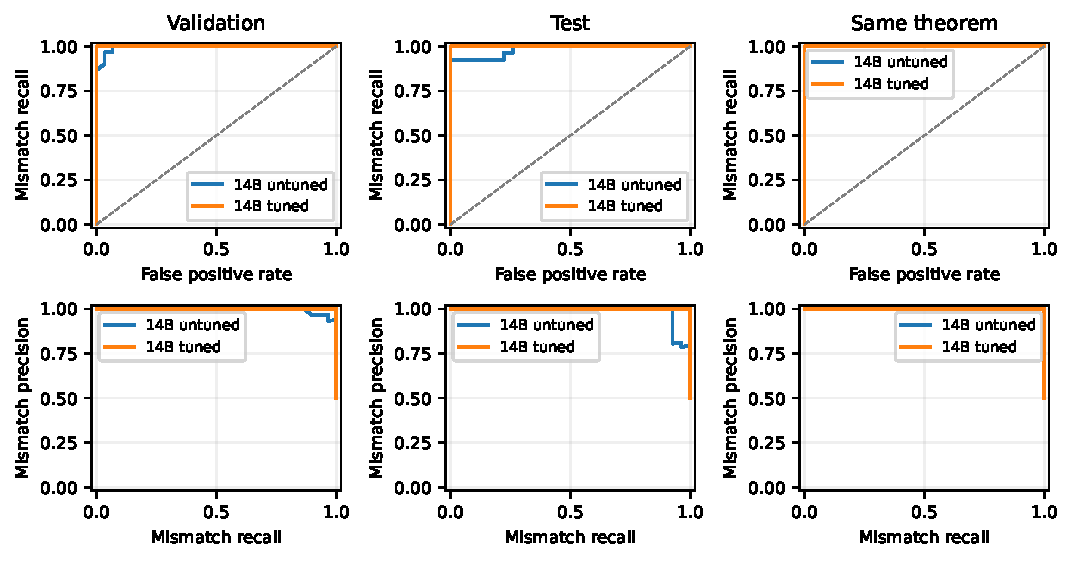
\includegraphics[width=\textwidth,height=.23\textheight,keepaspectratio]{figures/related-swap-curves.pdf}
\caption{Related-swap classifiers: ROC and precision--recall curves, with mismatch as the positive class. High ranking scores on the same-theorem diagnostic coexist with weaker fixed-threshold decisions. Other protocol figures remain in the supplement.}
\Description{ROC and precision-recall panels for original and related-swap-tuned Qwen14B.}
\label{fig:related}
\end{figure*}

\section{Main Experiment: Informalization}
\subsection{Separating translation from judgment}
\begin{figure}[t]
\centering
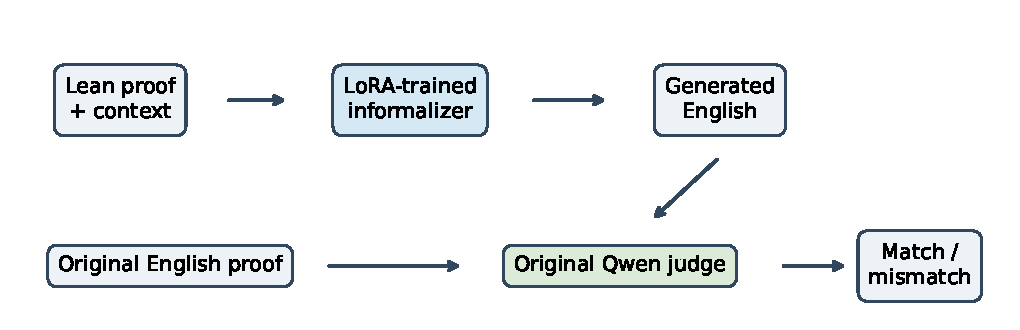
\includegraphics[width=\columnwidth]{figures/pipeline.pdf}
\caption{The original English enters only the comparison stage. The judge uses the original model with the informalization adapter disabled.}
\Description{Lean and context feed the trained informalizer; its English output and the original English feed the frozen comparison judge.}
\label{fig:pipeline}
\end{figure}
Let $L$ denote a Lean proof with its statement and supplied context, and $E$ the original English argument. Stage one produces an English account $\widehat E=T_\theta(L)$. Stage two returns a correspondence judgment $J(E,\widehat E)$. The translator never receives $E$ at inference time. This prevents it from simply reproducing the English argument that the judge is about to compare.

We train the translator to state assumptions and conclusions and explain the actual proof steps, witnesses, and dependencies. The prompt asks it to explain library lemmas as far as the supplied context supports and not invent a different proof. We optimize English completion tokens only; the Lean prompt is masked from the loss. This is supervised informalization, not classification training with match/mismatch labels.

The second stage uses the original Qwen3-14B base with the translation adapter disabled. Its input contains the original English theorem/proof and the generated account. The prompt allows paraphrases and routine elaboration, but rejects changed essential reasoning even when the conclusion is unchanged. We compare next-token logits for YES and NO. Their normalized score is uncalibrated and should not be read as a probability of mathematical truth. This stage receives no Lean text, making translation quality an explicit bottleneck.

\subsection{Herald training and held-out evaluation}
The base checkpoint is the publicly released Qwen3-14B model~\cite{qwen}.
We selected 4,096 original Herald pairs for training, 64 for validation, and 64 for testing. Splits were allocated by hashing connected components of declaration families, duplicate normalized English proofs, and duplicate formal signatures into 90/5/5 buckets, followed by capped seeded sampling. Exact reserved ProofNet proof/signature overlaps were excluded by the preparation procedure; this does not guarantee absence of conceptual overlap or shared dependencies.

We limited total training length to 2,048 tokens and English targets to 1,024. Oversized examples were excluded rather than truncated. This made the experiment manageable but selected for relatively short proofs. Qwen3-14B was loaded in BF16 without quantization. LoRA~\cite{lora} used rank 16, scaling 32, dropout 0.05, and attention query/key/value/output projections. Training used one epoch, learning rate $10^{-4}$, gradient accumulation of eight, and seed 883. Generation was greedy with thinking disabled and a 1,024-token output cap. The workstation used an RTX A6000 with 48 GB VRAM and 128 GB system memory.

The test applies both stages to held-out original pairs. It measures how often the judge accepts the translator's account, but has no newly adjudicated correspondence labels. A rejection can reflect a source-pair discrepancy, inaccurate informalization, or erroneous comparison. Validation completion loss measures fit to supplied English targets; it is not a semantic-equivalence metric. We report loss, output coverage, and acceptance separately from labeled classification metrics.

\subsection{ProofNet-supervised follow-up}
We trained a fresh adapter using the existing ProofNet proof pairs instead of Herald. It reuses the related-proof family allocation and the same length limits and hyperparameters. All eligible original training pairs are considered, not only examples that found a suitable swap. This leaves 176 training and 36 validation examples. Swapped negatives are never translation targets. We check disjoint family IDs and normalized English/Lean proof texts across splits.

The completed follow-up evaluates on the existing 54 related-swap test pairs and repeats the OpenAI cases. Validation completion NLL is 0.7276, compared with 0.2948 on Herald. The targets and populations differ, so these losses do not establish which translator is better. The difference in training-set size also prevents attributing a performance difference solely to dataset choice. Translation outputs that reach the generation limit are excluded from scored classification metrics, even when the raw judge subsequently produces a decision.

\section{Informalization Results}
\subsection{Held-out Herald behavior}
Figure~\ref{fig:informalization} shows training loss and the held-out decision counts. These describe optimization and model behavior, not an independent measure of semantic fidelity.
Training completed all 4,096 examples. All 64 held-out translations were nonempty and none hit the output limit. The English judge returned 49 MATCH and 15 MISMATCH, an acceptance rate of 76.56\%. Without independently checked labels, we cannot derive accuracy, a confusion matrix, or a meaningful semantic ROC curve for these judgments. Table~\ref{tab:informalization} separates these observations from labeled classification results.

Inspection of rejected outputs found translation errors, including an omitted cross-product contribution in an off-diagonal union argument and an incorrect explanation of permutation disjointness. This was exploratory inspection, not a blinded human evaluation. It nevertheless establishes why the 15 rejections cannot all be attributed to the original Lean--English pairs. Accepted outputs also require inspection: the judge may accept an account that changes a decisive step.

\begin{table}[t]
\centering\small
\caption{Herald-trained informalization observations. Acceptance is not accuracy.}
\label{tab:informalization}
\begin{adjustbox}{max width=\columnwidth}
\begin{tabular}{lr}
\toprule
Observation & Result \\
\midrule
Training / validation / test pairs & 4096 / 64 / 64 \\
Validation completion NLL & 0.2948 \\
Nonempty translations & 64/64 \\
Output-limit hits & 0/64 \\
English judge MATCH / MISMATCH & 49 / 15 \\
Independent test adjudication & Not performed \\
\bottomrule
\end{tabular}
\end{adjustbox}
\end{table}

\begin{figure*}[t]
\centering
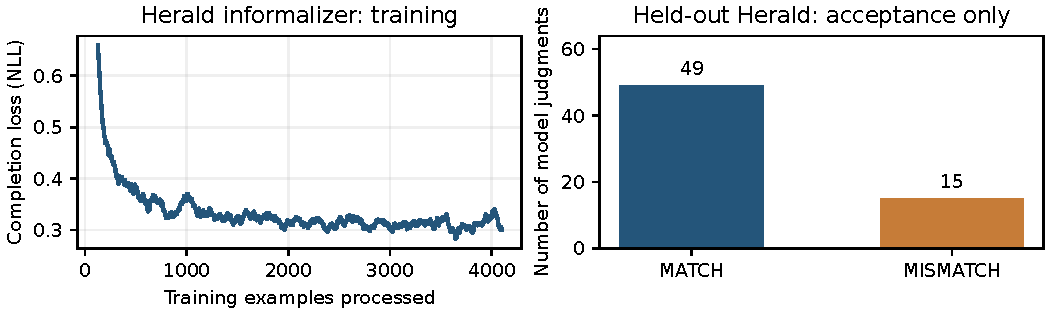
\includegraphics[width=.9\textwidth]{figures/informalization-herald.pdf}
\caption{Main Herald informalization experiment. Left: training completion loss, averaged over a trailing window of 128 examples. Right: decisions of the unchanged English judge on 64 held-out original pairs. The counts are acceptance/rejection, not correct/incorrect predictions.}
\Description{Training loss decreases over the epoch; the judge returns 49 matches and 15 mismatches.}
\label{fig:informalization}
\end{figure*}

\begin{figure*}[t]
\centering
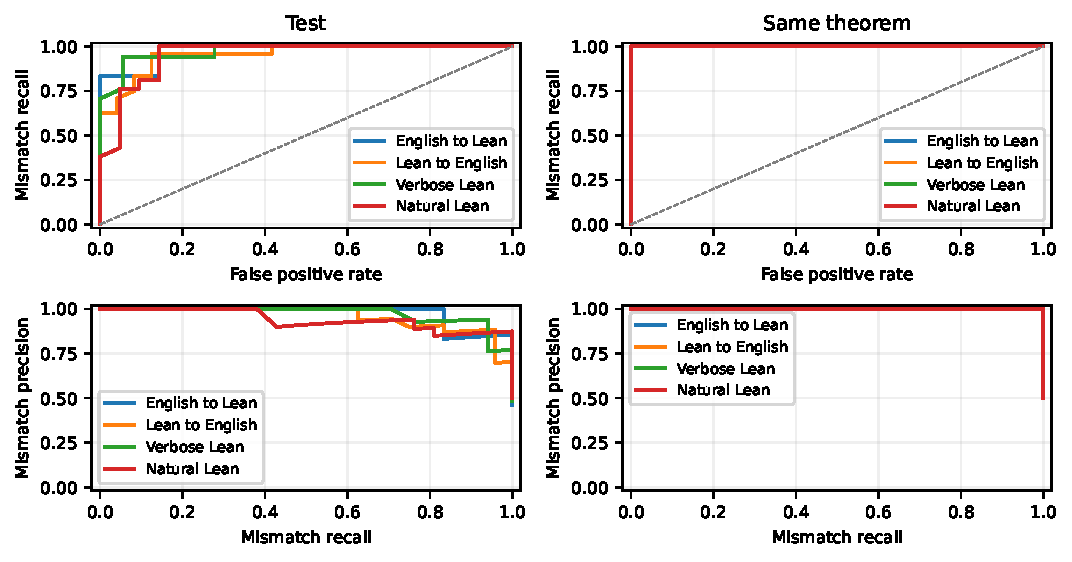
\includegraphics[width=\textwidth,height=.30\textheight,keepaspectratio]{figures/intermediaries-curves.pdf}
\caption{Earlier pretrained-14B intermediary experiment. These curves motivate the informalization study; they are not results for the Herald-trained translator. Scores are conditional on unequal coverage, and generated code pairs were not successfully verified.}
\Description{ROC and precision-recall curves for four intermediary architectures on related swaps and the small same-theorem diagnostic.}
\label{fig:intermediaries}
\end{figure*}

\subsection{ProofNet-trained pipeline on related swaps}
All 176 training examples completed, followed by 54 translations and 54 raw judgments. Eight translations reached the 1,024-token limit: both pairings for four source proofs, comprising four assumed matches and four synthetic mismatches. Treating these as abstentions leaves 46 scored pairs (85.19\% coverage). The pipeline correctly classifies 29/46, or 63.04\%. Mismatch precision is 0.575, recall is 1.000, and F1 is 0.730. The confusion matrix in Table~\ref{tab:main-confusion} is $[[23,0],[17,6]]$, with actual rows and predicted columns ordered as mismatch, match. Thus it rejects all 23 scored synthetic mismatches, but also rejects 17 of the 23 assumed matches.

The saved scores rank the classes better than the fixed decisions suggest: AUROC is 0.957 and average precision is 0.956 (Figure~\ref{fig:proofnet-informalization}). No threshold was fitted on this test. The earlier pretrained English-intermediary experiment scored 33/48 (68.75\%), compared with 29/46 here. These results do not demonstrate an improvement from ProofNet tuning, but the changed scored subsets and prompting protocols also prevent a controlled causal comparison. Neither percentage measures performance on independently human-labeled natural discrepancies.

\begin{figure}[t]
\centering
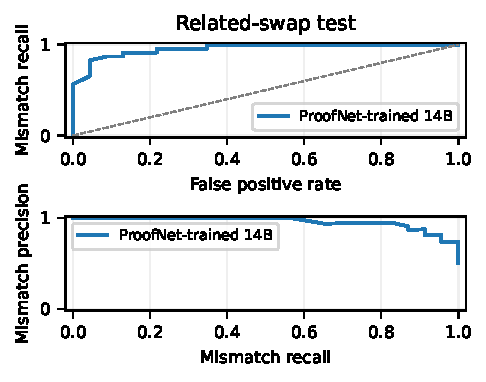
\includegraphics[width=\columnwidth]{figures/informalization-proofnet-curves.pdf}
\caption{ProofNet-trained informalization pipeline: ROC and precision--recall on 46 scored related-swap pairs; eight output-limit cases excluded. Mismatch is positive. Ranking scores do not remove the false rejections at the fixed decision boundary.}
\Description{ROC and precision-recall curves with AUROC 0.957 and average precision 0.956.}
\label{fig:proofnet-informalization}
\end{figure}

\subsection{OpenAI Navier--Stokes cases}
We selected two subarguments from the released manuscript and Lean repository~\cite{openaiproofs}, using revision \texttt{f9e8bc5} cited in the translation critique. The first is the inverse estimate in Lemma 8.6, equation (8.19), on pages 95--96. The second is the pressure-flux subargument of Lemma 10.5, ending at equation (10.19), on pages 121--123. We retained source hashes, visually checked the relevant equations, and prepared scoped English transcriptions. These are targeted subargument tests, not verification of the complete proof.

The Lean input includes the target declaration and selected definitions and helper bodies: 41 declarations across the cases, not a complete transitive dependency closure. Translator inputs contain 2,563 and 8,396 tokens, both outside the training-length regime. No input is truncated; the external output cap is 2,048 tokens. Neither stage receives the critique or expected labels. We separately request an explanatory judge response without conditioning it on the binary decision. No direct English--Lean baseline is run for these cases.

With the Herald-trained adapter, both receive MISMATCH and neither generation hits its limit. However, this does not demonstrate two correctly diagnosed source discrepancies. For the inverse estimate, the source comparison concerns an input requirement of $m+4$ versus $m+5$ derivatives. The translation retains Fourier coefficient inequalities but fails to explain what derivative assumptions its bound represents. The judge mainly contrasts derivative-word and seminorm terminology with the original inverse-operator description. Those notational differences are not themselves an adequate diagnosis.

For pressure flux, the translation describes a bound involving a cutoff norm and a dissipation root but leaves the bound as an unspecified expression. It explains the top-level wrapper rather than the supplied analytic helpers. The judge rejects missing detail, but does not identify the particular changed bound and analytic route. The result is compatible with noticing translation incompleteness rather than recovering the documented discrepancy. These selected cases contain no independently assessed faithful controls, and their explanations were reviewed by the AI collaborator rather than expert mathematical adjudicators. We report case outcomes, not general accuracy.

Repeating the same cases with the ProofNet-trained adapter does not resolve these failures. The inverse account ends after 27 tokens, saying only that a derivative of an inverse is bounded by a constant times a norm; it omits the argument and derivative requirement. The pressure account repeatedly states that the pressure difference is scalar and the velocity difference is a vector field, reaching the 2,048-token cap. Both raw judge decisions are MISMATCH, but the truncated pressure case is an abstention under our coverage policy. The explanations identify missing or repetitive content rather than the documented source discrepancies. Neither run therefore demonstrates reliable recovery of those discrepancies.

\subsection{Where information is lost}
A short Lean theorem can have a long mathematical argument distributed across dependencies. Translating only the surface sequence of tactics can produce a readable account that says little about the mathematics. Supplying helper code is insufficient if the model does not explain its assumptions and bounds. Stage two then compares a detailed source argument with an incomplete summary.

A faithful informalizer could still help human sanity checking even when the binary judge is unreliable. Our outputs do not establish that usefulness uniformly: omitted hypotheses or quantities can make readable prose misleading. A next version should translate helpers individually, preserve explicit assumptions and conclusions, and compose an account linked to Lean evidence. This would also help locate whether an error arose in the source pair, translation, or comparison.

\section{Limitations and Future Work}
\subsection{Experimental Result Takeaways}
The strongest classifier scores occur on constructed swaps. Original positives were assumed faithful, and a different source ID is not proof that a synthetic negative is semantically inequivalent. The same-theorem diagnostic is small and repeatedly inspected. Its success with several intermediaries is encouraging but not evidence of general performance on research mathematics. No result establishes superiority of controlled-language intermediaries over English: subsets differed, compilation failed, and the small diagnostic contained ties.

All main comparisons use local open-weight models. We did not perform a controlled frontier-model comparison, and openness alone is not an explanation for failure. Model size, data quality, effective context, generation budgets, and the objective are separate limitations. The 32B work demonstrates inference feasibility, not a successful larger-model fine-tune. The OpenAI cases also require more context than the short training examples.

The observations motivate the dataset problem, but do not prove it is the sole or dominant cause of every result. Threshold shifts and generation failures are visible counterexamples to that interpretation. The final pipeline is a heuristic aid to inspection, not an alternative trusted kernel or a certificate that an English argument is correct.

\subsection{A public human-reviewed correspondence database}
The most useful next resource would contain English--Lean pairs with human-reviewed correspondence labels and evidence for them. It should include faithful pairs and naturally occurring discrepancies from the same sources, so a model cannot identify the class simply from formatting, topic, or provenance. Examples should distinguish changed assumptions, domains, quantifiers, conclusions, witnesses, and steps. Same-theorem alternative routes are important, but are only one kind of mismatch.

Review should record more than a binary answer. Reviewers should point to the decisive English passage and Lean declaration, identify dependencies, and explain why a difference is substantive or presentational. Uncertain cases should remain uncertain. Multiple reviewers, disagreement records, and adjudication would make labels auditable. Human-checked positive pairs are particularly important: compiler acceptance cannot establish that the English explanation describes the checked proof.

The database should pin Lean and Mathlib versions, source revisions, extraction procedures, and licenses. Train/test separation should operate on theorem families and shared proofs, with independently maintained evaluation cases. Separate labels for statement fidelity, argument fidelity, and formal replay status would support whole-proof and step-level methods. Such data could evaluate informalization directly, rather than asking the same model family to certify its own translations.

Controlled representations remain a possible extension. A model might translate both sources into Verbose Lean, Natural Lean, or another structured account, with separate objectives for compilation and correspondence. Our experiments do not validate that architecture, but suggest why explicit intermediate claims and dependency structure are worth preserving. Transfer to Agda is another longer-term possibility once a reliable annotation and evaluation process exists.

\section{Conclusion}
We investigated checking whether English and Lean proofs preserve the same mathematical argument. Strong performance on synthetic swaps did not consistently transfer to subtle differences. Informalization can expose the Lean argument for comparison and reading, but introduces a failure point: essential information can disappear before the judge sees it. Our OpenAI case study produced mismatch flags without reliable identification of the reported discrepancies. Progress requires both better treatment of dependencies and public, human-reviewed faithful and unfaithful pairs. The goal is to help a reader understand what was proved and how, without confusing a learned judgment with formal verification.

\bibliographystyle{ACM-Reference-Format}
\bibliography{references}
\end{document}
